% Für Bindekorrektur als optionales Argument "BCORfaktormitmaßeinheit", dann
% sieht auch Option "twoside" vernünftig aus
% Näheres zu "scrartcl" bzw. "scrreprt" und "scrbook" siehe KOMA-Skript Doku
\documentclass[12pt,a4paper,titlepage,headinclude,bibtotoc]{scrartcl}


%---- Allgemeine Layout Einstellungen ------------------------------------------

% Für Kopf und Fußzeilen, siehe auch KOMA-Skript Doku
\usepackage[komastyle]{scrpage2}
\pagestyle{scrheadings}
\setheadsepline{0.5pt}[\color{black}]
\automark[section]{chapter}


%Einstellungen für Figuren- und Tabellenbeschriftungen
\setkomafont{captionlabel}{\sffamily\bfseries}
\setcapindent{0em}


%---- Weitere Pakete -----------------------------------------------------------
% Die Pakete sind alle in der TeX Live Distribution enthalten. Wichtige Adressen
% www.ctan.org, www.dante.de

% Sprachunterstützung
\usepackage[ngerman]{babel}

% Benutzung von Umlauten direkt im Text
% entweder "latin1" oder "utf8"
\usepackage[utf8]{inputenc}

% Pakete mit Mathesymbolen und zur Beseitigung von Schwächen der Mathe-Umgebung
\usepackage{latexsym,exscale,stmaryrd,amssymb,amsmath}

% Weitere Symbole
\usepackage[nointegrals]{wasysym}
\usepackage{eurosym}

% Anderes Literaturverzeichnisformat
%\usepackage[square,sort&compress]{natbib}

% Für Farbe
\usepackage{color}

% Zur Graphikausgabe
%Beipiel: \includegraphics[width=\textwidth]{grafik.png}
\usepackage{graphicx}
\usepackage{transparent}
% Text umfließt Graphiken und Tabellen
% Beispiel:
% \begin{wrapfigure}[Zeilenanzahl]{"l" oder "r"}{breite}
%   \centering
%   \includegraphics[width=...]{grafik}
%   \caption{Beschriftung} 
%   \label{fig:grafik}
% \end{wrapfigure}
\usepackage{wrapfig}

% Mehrere Abbildungen nebeneinander
% Beispiel:
% \begin{figure}[htb]
%   \centering
%   \subfigure[Beschriftung 1\label{fig:label1}]
%   {\includegraphics[width=0.49\textwidth]{grafik1}}
%   \hfill
%   \subfigure[Beschriftung 2\label{fig:label2}]
%   {\includegraphics[width=0.49\textwidth]{grafik2}}
%   \caption{Beschriftung allgemein}
%   \label{fig:label-gesamt}
% \end{figure}
\usepackage{subfigure}

% Caption neben Abbildung
% Beispiel:
% \sidecaptionvpos{figure}{"c" oder "t" oder "b"}
% \begin{SCfigure}[rel. Breite (normalerweise = 1)][hbt]
%   \centering
%   \includegraphics[width=0.5\textwidth]{grafik.png}
%   \caption{Beschreibung}
%   \label{fig:}
% \end{SCfigure}
\usepackage{sidecap}

% Befehl für "Entspricht"-Zeichen
\newcommand{\corresponds}{\ensuremath{\mathrel{\widehat{=}}}}

%Fußnoten zwingend auf diese Seite setzen
\interfootnotelinepenalty=1000

%Für chemische Formeln (von www.dante.de)
%% Anpassung an LaTeX(2e) von Bernd Raichle
%\makeatletter
%\DeclareRobustCommand{\chemical}[1]{%
%  {\(\m@th
%   \edef\resetfontdimens{\noexpand\)%
%       \fontdimen16\textfont2=\the\fontdimen16\textfont2
%       \fontdimen17\textfont2=\the\fontdimen17\textfont2\relax}%
%   \fontdimen16\textfont2=2.7pt \fontdimen17\textfont2=2.7pt
%   \mathrm{#1}%
%   \resetfontdimens}}
%\makeatother


\begin{document}

\begin{titlepage}
\centering
\textsc{\Large Anfängerpraktikum der Fakultät für
  Physik,\\[1.5ex] Universität Göttingen}

\vspace*{4.2cm}

\rule{\textwidth}{1pt}\\[0.5cm]
{\huge \bfseries
  Versuch Kreiselpräzession\\[1.5ex]
  Protokoll}\\[0.5cm]
\rule{\textwidth}{1pt}

\vspace*{3.5cm}

\begin{Large}
\begin{tabular}{ll}
Praktikant: &  Michael Lohmann\\
% &  Felix Kurtz\\
% &  Kevin Lüdemann\\
 &  Skrollan Detzler\\
 E-Mail: & m.lohmann@stud.uni-goettingen.de\\
% &  felix.kurtz@stud.uni-goettingen.de\\
% &  kevin.luedemann@stud.uni-goettingen.de\\
 &  skrollan.detzler@stud.uni-goettingen.de\\
 Betreuer: & Martin Ochmann\\
 Versuchsdatum: & 19.05.2014\\
\end{tabular}
\end{Large}

\vspace*{0.8cm}

\begin{Large}
\fbox{
  \begin{minipage}[t][2.5cm][t]{6cm} 
    Testat:
  \end{minipage}
}
\end{Large}

\end{titlepage}

\tableofcontents

\newpage

\section{Einleitung}
\label{sec:einleitung}
Kreisel spielen gerade in der Lagebestimmung eine große Rolle.
So besitzt nahezu jedes moderne Mobiltelefon Gyrosensoren, welche mithilfe von speziell gelagerten Kreiseln funktionieren.
Aber auch in der Astronomie spielen die hier beobachteten Effekte eine große Rolle.
So bewegt sich die Erde nicht genau auf einer Ellipse, sondern ''torkelt'' (wegen der Anziehungskraft des Mondes).
Dies lässt sich analog zu Kreiseln beschreiben.

\section{Theorie}
\label{sec:theorie}
Ein Kreisel ist ein Körper, der an einer Stelle gelagert ist.
Um diese kann er sich jedoch in allen Richtungen bewegen: z.B. in $\psi$- und $\vartheta$-Richtung, aber er kann auch um $\varphi$ rotieren.
Man kann so also erkennen, dass er insgesamt 3 Freiheitsgrade besitzt.
Um diese zu beschreiben, verwendet man gewöhnlicherweise die eulerschen Winkel.
Mit ihnen kann man den kompletten Zustand des Systems definieren.\\
Einen Kreisel, der symmetrisch ist bezüglich der sogenannten Figurenachse ist, welche durch den Befestigungspunkt und den Schwerpunkt verläuft, nennt man einen \emph{symmetrischen Kreisel}.\\
Man kann nun drei verschiedene Kegel der Kreiselbewegung sehen (s. Abb. \ref{img:kegel}): die Nutation um den Nutationskegel, Präzession um den Gangpolkegel und den Rastpolkegel.\\
Die Achse des Rastpolkegel ist die Richtung der Impulsachse, welche ohne Einwirkung äußerer Drehmomente konstant bleibt.
Der Gangpolkegel rollt sich mit einer festen Geschwindigkeit um den Rastpolkegel ab und deren Berührungslinie ist die momentane Rotationsachse.\\
Ein Kreisel heißt kräftefrei, wenn sich alle äußeren Drehmomente insgesamt aufheben.
Ein solcher Kreisel rotiert so lange konstant weiter, wie keine weiteren Drehmomente angreifen.


\begin{figure}[h]
\centering
\includegraphics[width=0.4\linewidth]{kegel.png}
\caption{verschiedene Kegel um die ein Kreisel sich bewegen kann\protect\footnotemark\label{img:kegel}}
\end{figure}
\footnotetext{https://lp.uni-goettingen.de/get/text/3637, 10.6.2014, 13 Uhr}
\subsection{Präzession}
Ein Kreisel, der waagerecht in der Luft hängt, ohne sich zu drehen, fällt durch die Schwerkraft nach unten.
Dreht er sich jedoch schnell genug, so beginnt er unter sonst gleichen Umständen, zu rotieren. Diese Bewegung nennt man Präzession.
Sie wird durch eine Kraft ausgelöst, welche senkrecht zum Drehimpuls $\vec L$ und zu dem daraus resultierenden Drehmoment $\vec M$ wirkt.
Die Präzessionsgeschwindigkeit $\omega_p$ ist die zeitliche Änderung des Winkels $\varphi$.
Außerdem gilt $d\varphi=\frac{dL}{L \cdot\sin\theta}=\frac{M\cdot dt}{L \cdot\sin\theta}$
\begin{align*}
\Rightarrow\:\omega_p=\frac{d\varphi}{dt}=\frac{M}{L \cdot\sin\theta}
\end{align*}
Außerdem gilt wegen $M=\vec{r}\times\vec{F}=m\vec{r}\times\vec{g}=m\cdot rg\sin\theta$ und $L=I\omega_k$ mit der Winkelgeschwindigkeit des Kreisels $\omega_k$
\begin{align}
\omega_p=\frac{m\cdot rg}{I\omega_k}
\end{align}


\subsection{Nutation}

Da der Massenmittelpunkt sich bewegt, wirkt ein kleines Drehmoment, welches nach oben wirkt.
Dadurch fällt die momentane Drehachse nicht mehr mit der Figurenachse zusammen, sondern sie rotiert auf dem Nutationskegel um diese herum.
Diese Bewegung nennt man \emph{Nutation}.\\
Man kann nun den Drehimpuls aufteilen in Komponenten, die parallel und orthogonal zur momentanen Drehachse sind: $\vec L=\vec L_{||}+\vec L_\perp=I\vec\omega_{||}+I\vec\omega_\perp$. Da $|L|=\frac{|L_{||}|}{\cos\varphi}=\frac{L_\perp}{\sin\varphi}$ gilt für die Nutationswinkelgeschwindigkeit $\omega_N$:
\begin{align*}
|\vec{\omega_N}|=\frac{\omega_\perp}{\sin\varphi}=\frac{I_{||}\cdot\omega_{||}}{I_\perp\cos\varphi}
\end{align*}
Da $\varphi\approx 0\Rightarrow \cos\varphi\approx 1$
\begin{align}
\omega_N\approx\frac{I_{||}}{I_\perp}\omega
\end{align}

% \subsection{Corioliskraft}
%Eines der wichtigsten Phänomene der Corioliskraft ist die haupsächliche Windrichtung der globalen Luftströmungen auf der Erde.
%So ist diese auf der Nordhalbkugel ostwärts, während sie auf der Südhalbkugel dem entgegengerichtet ist.

 
\section{Durchführung}
\label{sec:durchfuehrung}
 \begin{figure}[!htb]
 \centering \def\svgwidth{100pt}
 \input{bild1.pdf_tex}
\caption{Bezeichnungen der wichtigen Größen\label{img:wichtigegr}}
 \end{figure}
Zu Beginn werden die Maße des Kreisels bestimmt.
Danach schraubt man das Zusatzgewicht in eines der dafür vorgesehenen Löcher am äußeren Rand der Kreisscheibe.
Nun nimmt man 3 mal hintereinander die Zeit, die das System benötigt, um 10 Schwingungen bei kleiner Auslenkung zu vollziehen, bei eingespannter Halterung.
Dies wiederholt man noch einmal mit dem Zusatzgewicht diametral auf der anderen Seite der Scheibe angebracht.\\
Für den nächsten Teilversuch wird die Einspannung gelöst, so dass sich der Kreisel frei um den Ständer drehen kann.
Das Ausgleichsgewicht sollte nun so befestigt sein, dass sich der Kreisel in der Schwebe hält, wodurch dieser zu einem kräftefreien wird.
Nun wird der Kreisel mithilfe eines Seils in schnelle Rotation versetzt.
Unter Zuhilfenahme einer Lichtschranke wird die Rotationsfrequenz gemessen.
Ein Zusatzgewicht wird nun an das Ende der Stange zum Ausgleichsgewicht gehängt und dabei ist zu beobachten, dass der Kreisel beginnt, sich um die Aufhängung zu drehen.
Nach jeweils einer halben Drehung wird das Zusatzgewicht vorsichtig abgenommen und die Rotationsfrequenz des Rades erneut bestimmt.
Dies wiederholt man so häufig wie möglich und alles zusammen noch 2 mal.\\
Für den letzten Teilversuch wird der Kreisel wie oben in schnelle Rotation versetzt und dann die Winkelgeschwindigkeit gemessen.
Dann wird ihm einen kräftiger Schlag auf die Achse gegeben.
Dies führt zu einer Nutation, deren durchschnittliche Periodenlänge über mehrere Perioden gemessen wird.
Auch dieser Versuchsteil wird mehrfach wiederholt.


\section{Auswertung}
\label{sec:auswertung}

\subsection{Trägheitsmoment des Rades}
Das Trägheitsmoment eines Rades in horizontaler Richtung beträgt $$I_{hor}=\dfrac{1}{2}mr^2$$
Mit einer Masse m von $1.324$ kg und einem Radius $r=0.1225$m ergibt sich $I_{hor}=9.93\cdot 10^{-3}$kg m$^2$\\
Das Trägheitsmoment der gesamten Konstruktion errechnet sich aus
\begin{align*}
I_z&=I_{Ausgl.Gew.}+I_{Stab}+I_{Rad}\\
&= m_gz_g^2+\dfrac{1}{12}m_sl^2+m_sd_s^2+\dfrac{1}{4}m_rr^2+\dfrac{1}{12}m_rd^2+m_rz_r^2
\end{align*}
Dies wurde mithilfe des Hebelgesetzes und des Satzes von Steiner, sowie mit der Masse des Ausgleichsgewichts $m_g=0.936$kg, dessen Entfernung zur Drehachse $z_g=(0.17\pm 0.01)$m, der Masse des Stabes $m_s=(0.4\pm 0.2)$kg, seiner Länge $l=(0.48\pm 0.005)$m und dem Abstand seines CM zur Drehachse $d_s=(0.10\pm 0.01)$m berechnet. Außerdem der Masse des Rades $m_r=1.324$kg mit seinem Durchmesser $d$ und dessen Abstand zur Drehachse $z_r=0.12$m. Die Masse des Stabes, welche weder gegeben war, noch vermessen werden konnte, wurde so grob auf $0.4$kg geschätzt, was in einem großen Fehler dieser Messgröße resultiert.
Insgesamt ergibt sich ein Wert von $I_z=64.5\cdot 10^{-3}$kg m$^2$.


\subsection{Pendel}
Nach dem Versuch 3 (Das Trägheitsmoment) gilt: $$I=\dfrac{T^2gmz}{4\pi^2}-mz^2$$

Der Fehler wurde mit der Gaußschen Fehlerfortpflanzung berechnet:
$$\sigma_I=\sqrt{\sigma_T^2\left(\dfrac{\partial I}{\partial T}\right)^2}=\sqrt{\left(\dfrac{\sigma_T\cdot Tmgz}{2\pi^2}\right)^2}$$
Die Werte werden in Abbildung \ref{img:pendeldaten} dargestellt.\\
Insgesamt ergibt sich so aus Tabelle \ref{tab:pendel} ein Trägheitsmoment von \(I=(8.7\pm 0.02)\cdot 10^{-3}\text{kg m}^2\).
\begin{table}[h!]
\centering
\begin{tabular}{|c|c|}
\hline 
$T$ [s] & $I$ [$10^{-3}\cdot \text{kg m}^2$] \\ 
\hline 
$2.01\pm 0.03$ & $(8.6\pm 0.03)$ \\ 
\hline 
$2.03\pm 0.03$ & $(8.8\pm 0.03)$\\ 
\hline
$2.03\pm 0.03$ & $(8.8\pm 0.03)$ \\ 
\hline 
$2.02\pm 0.03$ & $(8.7\pm 0.03)$ \\ 
\hline 
$2.02\pm 0.03$ & $(8.7\pm 0.03)$ \\ 
\hline 
$2.02\pm 0.03$ & $(8.7\pm 0.03)$ \\ 
\hline 
\end{tabular}
\caption{Trägheitsmoment des Pendels\label{tab:pendel}}
\end{table}
\begin{figure}
\centering
% GNUPLOT: LaTeX picture with Postscript
\begingroup
  \makeatletter
  \providecommand\color[2][]{%
    \GenericError{(gnuplot) \space\space\space\@spaces}{%
      Package color not loaded in conjunction with
      terminal option `colourtext'%
    }{See the gnuplot documentation for explanation.%
    }{Either use 'blacktext' in gnuplot or load the package
      color.sty in LaTeX.}%
    \renewcommand\color[2][]{}%
  }%
  \providecommand\includegraphics[2][]{%
    \GenericError{(gnuplot) \space\space\space\@spaces}{%
      Package graphicx or graphics not loaded%
    }{See the gnuplot documentation for explanation.%
    }{The gnuplot epslatex terminal needs graphicx.sty or graphics.sty.}%
    \renewcommand\includegraphics[2][]{}%
  }%
  \providecommand\rotatebox[2]{#2}%
  \@ifundefined{ifGPcolor}{%
    \newif\ifGPcolor
    \GPcolortrue
  }{}%
  \@ifundefined{ifGPblacktext}{%
    \newif\ifGPblacktext
    \GPblacktexttrue
  }{}%
  % define a \g@addto@macro without @ in the name:
  \let\gplgaddtomacro\g@addto@macro
  % define empty templates for all commands taking text:
  \gdef\gplbacktext{}%
  \gdef\gplfronttext{}%
  \makeatother
  \ifGPblacktext
    % no textcolor at all
    \def\colorrgb#1{}%
    \def\colorgray#1{}%
  \else
    % gray or color?
    \ifGPcolor
      \def\colorrgb#1{\color[rgb]{#1}}%
      \def\colorgray#1{\color[gray]{#1}}%
      \expandafter\def\csname LTw\endcsname{\color{white}}%
      \expandafter\def\csname LTb\endcsname{\color{black}}%
      \expandafter\def\csname LTa\endcsname{\color{black}}%
      \expandafter\def\csname LT0\endcsname{\color[rgb]{1,0,0}}%
      \expandafter\def\csname LT1\endcsname{\color[rgb]{0,1,0}}%
      \expandafter\def\csname LT2\endcsname{\color[rgb]{0,0,1}}%
      \expandafter\def\csname LT3\endcsname{\color[rgb]{1,0,1}}%
      \expandafter\def\csname LT4\endcsname{\color[rgb]{0,1,1}}%
      \expandafter\def\csname LT5\endcsname{\color[rgb]{1,1,0}}%
      \expandafter\def\csname LT6\endcsname{\color[rgb]{0,0,0}}%
      \expandafter\def\csname LT7\endcsname{\color[rgb]{1,0.3,0}}%
      \expandafter\def\csname LT8\endcsname{\color[rgb]{0.5,0.5,0.5}}%
    \else
      % gray
      \def\colorrgb#1{\color{black}}%
      \def\colorgray#1{\color[gray]{#1}}%
      \expandafter\def\csname LTw\endcsname{\color{white}}%
      \expandafter\def\csname LTb\endcsname{\color{black}}%
      \expandafter\def\csname LTa\endcsname{\color{black}}%
      \expandafter\def\csname LT0\endcsname{\color{black}}%
      \expandafter\def\csname LT1\endcsname{\color{black}}%
      \expandafter\def\csname LT2\endcsname{\color{black}}%
      \expandafter\def\csname LT3\endcsname{\color{black}}%
      \expandafter\def\csname LT4\endcsname{\color{black}}%
      \expandafter\def\csname LT5\endcsname{\color{black}}%
      \expandafter\def\csname LT6\endcsname{\color{black}}%
      \expandafter\def\csname LT7\endcsname{\color{black}}%
      \expandafter\def\csname LT8\endcsname{\color{black}}%
    \fi
  \fi
  \setlength{\unitlength}{0.0500bp}%
  \begin{picture}(7200.00,5040.00)%
    \gplgaddtomacro\gplbacktext{%
      \csname LTb\endcsname%
      \put(1474,704){\makebox(0,0)[r]{\strut{} 0.00855}}%
      \csname LTb\endcsname%
      \put(1474,1382){\makebox(0,0)[r]{\strut{} 0.0086}}%
      \csname LTb\endcsname%
      \put(1474,2061){\makebox(0,0)[r]{\strut{} 0.00865}}%
      \csname LTb\endcsname%
      \put(1474,2739){\makebox(0,0)[r]{\strut{} 0.0087}}%
      \csname LTb\endcsname%
      \put(1474,3418){\makebox(0,0)[r]{\strut{} 0.00875}}%
      \csname LTb\endcsname%
      \put(1474,4096){\makebox(0,0)[r]{\strut{} 0.0088}}%
      \csname LTb\endcsname%
      \put(1474,4775){\makebox(0,0)[r]{\strut{} 0.00885}}%
      \csname LTb\endcsname%
      \put(1606,484){\makebox(0,0){\strut{} 0}}%
      \csname LTb\endcsname%
      \put(2348,484){\makebox(0,0){\strut{} 1}}%
      \csname LTb\endcsname%
      \put(3091,484){\makebox(0,0){\strut{} 2}}%
      \csname LTb\endcsname%
      \put(3833,484){\makebox(0,0){\strut{} 3}}%
      \csname LTb\endcsname%
      \put(4576,484){\makebox(0,0){\strut{} 4}}%
      \csname LTb\endcsname%
      \put(5318,484){\makebox(0,0){\strut{} 5}}%
      \csname LTb\endcsname%
      \put(6061,484){\makebox(0,0){\strut{} 6}}%
      \csname LTb\endcsname%
      \put(6803,484){\makebox(0,0){\strut{} 7}}%
      \put(176,2739){\rotatebox{-270}{\makebox(0,0){\strut{}Trägheitsmoment [kg m$^2$]}}}%
      \put(4204,154){\makebox(0,0){\strut{}Messung}}%
    }%
    \gplgaddtomacro\gplfronttext{%
      \csname LTb\endcsname%
      \put(5816,4602){\makebox(0,0)[r]{\strut{}'Pendel.dat'}}%
      \csname LTb\endcsname%
      \put(5816,4382){\makebox(0,0)[r]{\strut{}Mittelwert}}%
    }%
    \gplbacktext
    \put(0,0){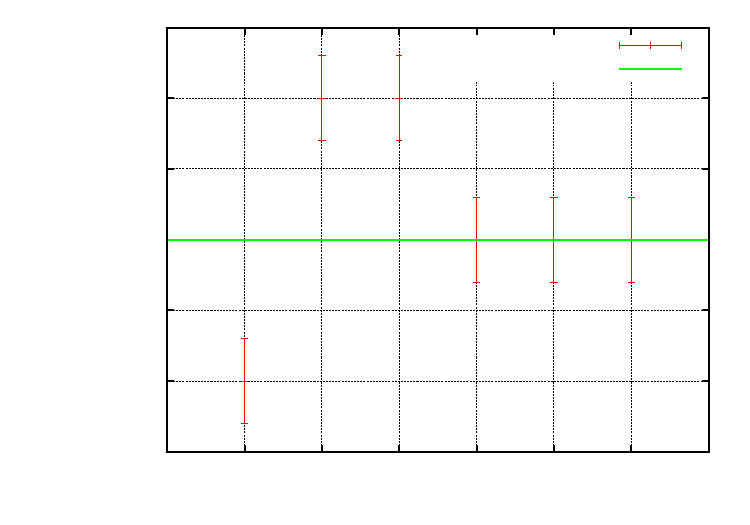
\includegraphics{pendeldaten}}%
    \gplfronttext
  \end{picture}%
\endgroup

\caption{Trägheitsmomente aus dem Pendelversuch\label{img:pendeldaten}}
\end{figure}


\subsection{Präzession}
\begin{figure}[!htb]
\centering
\include{MessungPraezession.tex}
\caption{Präzessionswerte}
\end{figure}

\subsection{Nutation}



\section{Diskussion}
\label{sec:diskussion}
Das Gewicht der Stange ließ sich nicht bestimmen, ohne die komplette Apparatur auseinanderzubauen.
Dies ist natürlich nicht wünschenswert und so fehlte uns leider dieser Wert zur genaueren Berechnung.
Ein Vermerk auf der Stange selber oder im Handbuch wäre diesbezüglich hilfreich.
Auch war die Messung der verschiedenen Abstände nicht immer einfach zu messen, da das Lineal nicht eben anzulegen war.


\end{document}
